\chapter{Mathematical Preliminaries}
\label{chapter:mathematical-preliminaries}

This chapter is intended to serve as a reference point for the more fundemental concepts that are used throughout this dissertation. In particular, this dissertation contains a signficant amount of  discussion on \textit{Formal Concept Analysis} and \textit{Preference Relations}; which, in turn, are based on order theory, which is where we begin. The second half of this chapter provides an introduction to basic notions in logic, given in the setting of propositional logic.

\section{Order and Lattice Theory}
\label{section:order-theory}

\begin{definition}
  \label{definition:binary-relation}
  A \textbf{binary relation} \index{binary relation} $R$ over two sets $X$ and $Y$ is a set of pairs $(x,y)$ with $x \in X$ and $y \in Y$; and so $R \subseteq X \times Y$. In many cases we express this pair using infix notation, and we write $xRy$.
\end{definition}

Binary relations are not particularly interesting until they satisfy certain properties. We now discuss certain binary relations which occur frequently enough to deserve a distinct name.

\begin{definition}
  \label{definition:partial-order}
  A \textbf{partial-order} \index{partial-order} is a binary relation $\preceq \; \subseteq X \times X$ that satisfies the following properties:
  \begin{align}
    & \text{(Reflexivity)} & x \preceq x \\
    & \text{(Antisymmetry)} & x \preceq y \text{ and } y \preceq x \text{ implies } x = y \\
    & \text{(Transitivity)} & x \preceq y \text{ and } y \preceq z \text{ implies } x \preceq z
  \end{align}
  for all $x,y,z \in X$.
\end{definition}

We write $x \npreceq y$ to indicate that $x \preceq y$ does not hold, and $x \prec y$ for the case where $x\preceq y$ and $x \not = y$. When $x \not \preceq y$ and $y \not \preceq x$---i.e., that $x$ and $y$ are incomparable---we write $x \Vert y$ \cite{Davey_Priestley_2002}. From a partial-order we can quite easily induce the notion of a \emph{strict partial-order}.

\begin{definition}
  \label{definition:strict-partial-order}
  A \textbf{strict partial-order} \index{strict partial-order} is a binary relation $\prec \; \subseteq X \times X$ that satisfies:
  \begin{align}
    & \text{(Irreflexivity)} & x \nprec x \\
    & \text{(Asymmetry)} & x \prec y \text{ implies } y \nprec x \\
    & \text{(Transitivity)} & x \prec y \text{ and } y \prec z \text{ implies } x \prec z
  \end{align}
  for all $x,y,z \in X$.
\end{definition}

An ordered set is a pair $(X, \preceq)$ with $X$ being a set and $\preceq$ being an ordering on $X$. If $\preceq$ is a partial-ordering, we might then refer to $X$ as a \textit{poset}.

\begin{figure}[H]
  \label{figure:hasse-diagram}
  \centering
  \begin{subfigure}{0.3\textwidth}
    \centering
    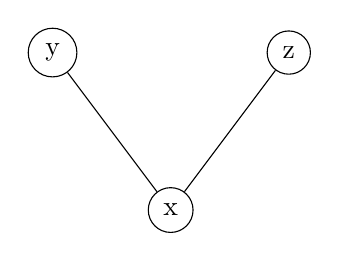
\begin{tikzpicture}[every node/.style={circle, draw, minimum size=0.25cm}]
      \node (y) at (-1.5,0) {y};
      \node (z) at (1.5,0) {z};
      \node (x) at (0,-2) {x};

      \draw (y) -- (x);
      \draw (z) -- (x);
    \end{tikzpicture}
    \subcaption{$\preceq_a$}
    \label{subfigure:partial-order-a}
  \end{subfigure}%
  \begin{subfigure}{0.3\textwidth}
    \centering
    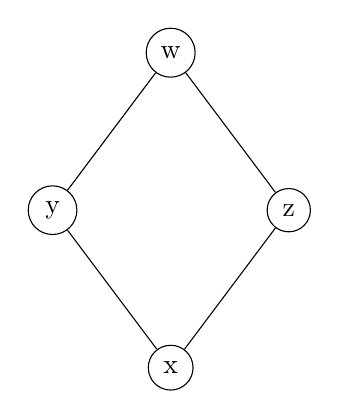
\begin{tikzpicture}[every node/.style={circle, draw, minimum size=0.25cm}]
      \node (w) at (0,2) {w};
      \node (y) at (-1.5,0) {y};
      \node (z) at (1.5,0) {z};
      \node (x) at (0,-2) {x};

      \draw (w) -- (y);
      \draw (w) -- (z);
      \draw (y) -- (x);
      \draw (z) -- (x);
    \end{tikzpicture}
    \subcaption{$\preceq_b$}
    \label{subfigure:partial-order-b}
  \end{subfigure}%
  \begin{subfigure}{0.3\textwidth}
    \centering
    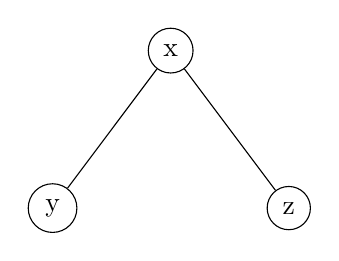
\begin{tikzpicture}[every node/.style={circle, draw, minimum size=0.25cm}]
      \node (y) at (-1.5,0) {y};
      \node (z) at (1.5,0) {z};
      \node (x) at (0,2) {x};

      \draw (y) -- (x);
      \draw (z) -- (x);
    \end{tikzpicture}
    \subcaption{$\preceq_a$}
    \label{subfigure:partial-order-c}
  \end{subfigure}%
  \caption{Three partial-orders over a set $P$}
\end{figure}

% A \emph{binary relation} \index{binary relation} on a set $P$ is a subset $\prec \; \subseteq P \times P$. Then, a binary relation that satisfies the following two conditions is called a \textit{strict partial-order} \index{strict partial-order}, where $x,y,$ and $z$ are elements of $P$
% \begin{align}
%   x \prec y \text{ and } y \prec z \text{ implies } x \prec z \\
%   x \prec y \text{ implies } y \not \prec x
% \end{align}

% In other words, a strict partial-order is a binary relation that is both \textit{transitive} (1.1) and \textit{asymemtric} (1.2). Under these conditions, a strict partial-order is also \textit{irreflexive} (1.3)
% \begin{align}
%   x \not \prec x
% \end{align}

% A (non-strict) partial-order \index{partial-order} is a binary relation, $\preceq \; \subseteq P \times P$, that satisfies \textit{reflexivity} (1.4), \textit{transitivity} (1.5), and \textit{antisymmetry} (1.6) \cite{Davey_Priestley_2002}.
% \begin{align}
%   x \preceq x \\
%   x \preceq y \text{ and } y \preceq z \text{ implies } x \preceq z \\
%   x \preceq y \text{ and } y \preceq x \text{ implies } x = y
% \end{align}

% We can represent a partially-ordered set diagramatically with a \textit{Hasse diagram} \index{Hasse diagram}. Then,

% \begin{figure}[H]
%   \label{figure:hasse-diagram}
%   \centering
%   \begin{subfigure}{0.3\textwidth}
%     \centering
%     \begin{tikzpicture}[every node/.style={circle, draw, minimum size=0.25cm}]
%       \node (y) at (-1.5,0) {y};
%       \node (z) at (1.5,0) {z};
%       \node (x) at (0,-2) {x};

%       \draw (y) -- (x);
%       \draw (z) -- (x);
%     \end{tikzpicture}
%     \subcaption{$\preceq_a$}
%     \label{subfigure:partial-order-a}
%   \end{subfigure}%
%   \begin{subfigure}{0.3\textwidth}
%     \centering
%     \begin{tikzpicture}[every node/.style={circle, draw, minimum size=0.25cm}]
%       \node (w) at (0,2) {w};
%       \node (y) at (-1.5,0) {y};
%       \node (z) at (1.5,0) {z};
%       \node (x) at (0,-2) {x};

%       \draw (w) -- (y);
%       \draw (w) -- (z);
%       \draw (y) -- (x);
%       \draw (z) -- (x);
%     \end{tikzpicture}
%     \subcaption{$\preceq_b$}
%     \label{subfigure:partial-order-b}
%   \end{subfigure}%
%   \begin{subfigure}{0.3\textwidth}
%     \centering
%     \begin{tikzpicture}[every node/.style={circle, draw, minimum size=0.25cm}]
%       \node (z) at (0,2) {z};
%       \node (y) at (0,0) {y};
%       \node (x) at (0,-2) {x};
%       \node (w) at (1.5,0) {w};

%       \draw (x) -- (y);
%       \draw (y) -- (z);
%     \end{tikzpicture}
%     \subcaption{$\preceq_c$}
%     \label{subfigure:partial-order-c}
%   \end{subfigure}
%   \caption{Three partial-orders over a set $P$}
% \end{figure}
